\documentclass[12pt]{article}
\usepackage[margin=1in]{geometry}
\usepackage[framemethod=default]{mdframed}
\usepackage{amsmath, amsthm, amsfonts, tikz, algpseudocode}

\theoremstyle{plain}
\newtheorem*{theorem}{Theorem}
\newtheorem*{lemma}{Lemma}
\newtheorem*{claim}{Claim}
\newtheorem*{definition}{Definition}
\newtheorem*{corollary}{Corollary}


\usepackage[plain]{algorithm}

%%%% TITLE

\title{Bayesian optimization of\\TRPO using Gaussian Processes}
\date{April 21}
\author{Yixin Lin}

\begin{document}
\maketitle

\begin{abstract}
  Trust region policy optimization is a popular reinforcement learning algorithm with theoretical guarantees on monotonic policy improvement. We explore applying Bayesian hyperparameter optimization on the size of the trust region. We notice potential gains but lose some of the theoretical guarantees.
\end{abstract}

\part{Introduction}

\section{Motivation}

Trust region policy optimization (or TRPO) is a reinforcement learning algorithm which is a policy gradient approach that uses natural gradients. Though it has proven both successful on a wide variety of tasks and scalable to large amounts of policy parameters, one issue that it (and policy gradient approaches in general) is that it is highly sample inefficient. This means that though there are theoretical convergence guarantees, in practice it may take a long time to reach convergence and require many simulations.

\section{Problem definition} 

Trust region policy optimization is a reinforcement learning algorithm which attempts to optimize a policy $ \pi(a|s) $
in order to maximize the standard $Q$-function $ Q^\pi(s,a) = r + \gamma \max Q^\pi(s',a') $
and it does this by assuming a parameterized policy $\pi_\theta$, iteratively improving the policy by optimizing the parameters subject to a maximum KL divergence which is controlled by a hyperparameter $\delta$. This is then approximated by linearization and a Monte Carlo sampling approach.

Our goal is to optimize this using method by using ideas from Bayesian optimization of hyperparameters, e.g. in the Snoek paper we read in class, to optimize the hyperparameters used in each iteration. Specifically, we have the hyperparameters $\delta$ as well as the number of timesteps of data per iteration which can both be optimized every iteration in the way described in the paper.



\part{Preliminaries}

\section{``Trust Region Policy Optimization'', Schulman et al.}

Policy gradient methods work by attempting to directly optimize a parameterized policy $\pi$.  First, these methods sample trajectories through state-space using some randomly initialized $\pi_0$, estimating a gradient to the policy, and taking a step in that direction.

Schulman extends the 2002 Kakade and Langford paper on the conservative policy iteration method by extending it to work for all general stochastic policy classes. Specifically, in Kakade and Langford, the expected cost of a policy, defined as $\eta(\pi) = \mathbb{E} [ \sum_{t=0}^\infty \gamma^t c(s_t)]$, is optimized through a local approximation

$$ L_\pi(\tilde{\pi}) = \eta(\pi) + \sum_s \rho_\pi (s) \sum_a \tilde{\pi} (a|s) A_\pi (s,a) $$

where the state visitation frequency $\rho_\tilde{\pi}$ of the new policy is replaced by the known visitation frequency $\rho_\pi$. Kakade and Langford proved that optimizing this objective with gradient descent will improve $\eta$ monotonically, if the step taken is small enough.

% Schulman extends this to arbitrary stochastic policy classes by using the total variation divergence, which is bounded by the $KL$ divergence; thus, they provide a theoretical guarantee of monotonic policy improvement. This is similar to previous natural policy gradient methods, which place a penalty term on the KL divergence of the old and new policies in order to regularize the loss.

Schulman then derives a practical algorithm, called Trust Region Policy Optimization, which uses a constraint on the KL divergence instead of a penalty term. Though they use approximations and substitutions for practical reasons, the algorithm is shown to work empirically quite well and close to the theoretically-guaranteed results. This is shown on robot locomotion simulation tasks, using a single value of the hyperparameter $\delta$ (the constant that limits the amount of KL divergence) worked well, as well as Atari games, where it performed decently without significant problem-specific engineering.

The main takeaway is that the TRPO algorithm is quite generalizable and easy to tune, and provides a great baseline policy gradient algorithm.

\begin{figure}[h]
  \centering
  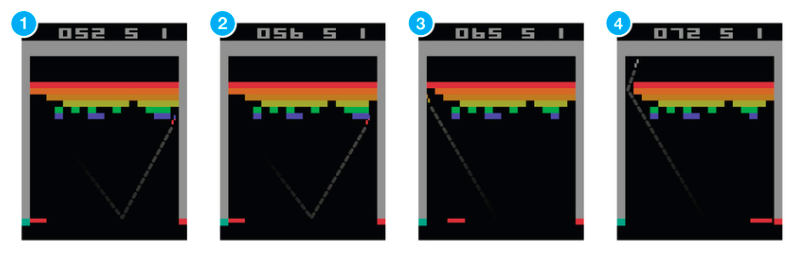
\includegraphics[width=0.5\textwidth]{atari.png}
  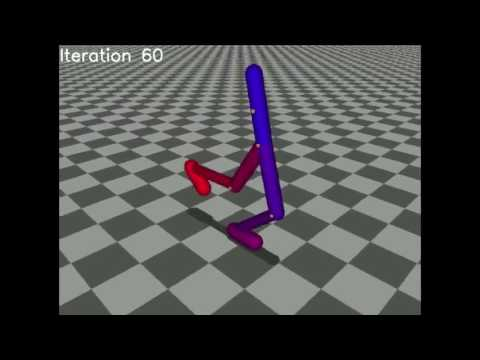
\includegraphics[width=0.4\textwidth]{walker.jpg}
  \caption{The Atari and Walker environments upon which TRPO was trained in the original paper.}
\end{figure}

\section{Gaussian Processes}

A \textit{Gaussian process} is a collection of random variables, any finite number of which have a joint Gaussian distribution. The mean function $m(\bold{x})$ and covariance function (kernel) $k(\bold{x}, \bold{x}^{'} )$ uniquely defines it. A simple way to see it is in the finite index sets, ``which would be simply Gaussian \textit{distributions}'': essentially, each $x$ has a distribution around it. Taking the limit for $x \in \mathcal{R}$ results in the Gaussian process. Given a finite dataset of $X, f(X)$, the Gaussian process fits to the function with low variance around the given datasets and opposite for the extrapolation.

\begin{figure}[h]
  \centering
  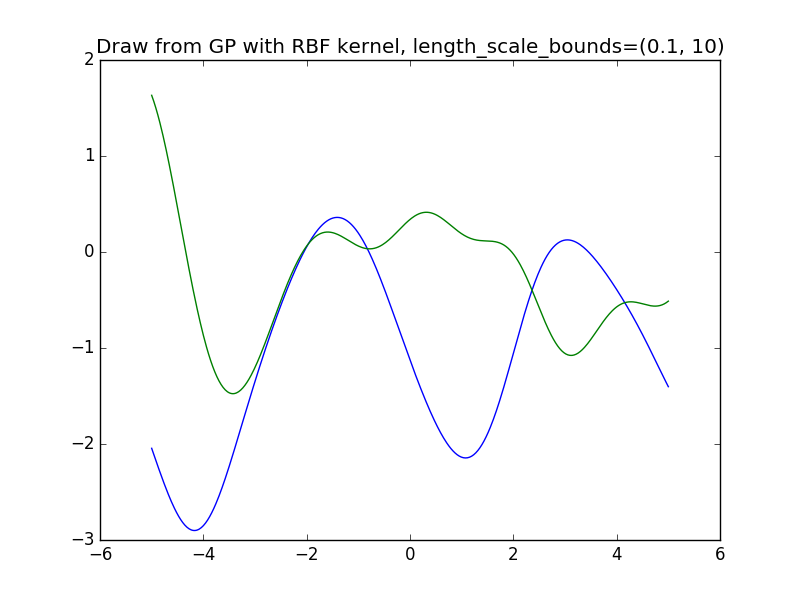
\includegraphics[width=0.5\textwidth]{gp1.png}

  \caption{Examples of draws from Gaussian processes}
\end{figure}


\section{``Practical bayesian optimizations of machine learning algorithms'', Snoek et al.}

% Snoek uses a Bayesian Gaussian process approach for the problem of tuning hyperparameters of machine learning algorithms. Hyperparameter tuning inevitably makes a huge difference in model performance and generalizability but is often an inefficient, art-not-a-science style of activity.

Snoek provides a set of good practices for Bayesian hyperparameter optimization. The model is a Gaussian Process for the hyperparameters, which they recommend tuning using a Bayesian treatment. Generally, the tradeoff for optimization problems is whether to use simple local information (e.g. gradient and Hessian computations) for a fast iterations, or performing a more complicated iterative steps (e.g. by using all previous evaluations) in order to have less iterations. Since the process of optimizing a machine learning algorithm's hyperparameters requires the use of 1. training a machine learning algorithm, and 2. running it on test data, this process is extremely computationally intense, which means that having a complex (i.e. fully Bayesian) computation for the next hyperparameter to try is worth it.

% The idea behind their version of Bayesian optimization is that it constructs a probabilistic approximation of $f(\mathbf{x})$, the function to be optimized, and uses it (i.e. all historical data) to figure out what parameters to try next. First, we must choose a prior. They choose a Gaussian prior due to its extreme flexibility and tractability, and choose an \textit{acquisition function} which is used to choose the next point to evaluate.

% $K_{M52}(\mathbf{x}, \mathbf{x}') = \theta_0(1 + \sqrt{5r^2 (\mathbf{x}, \mathbf{x}')} + \frac{5}{3} r^2(\mathbf{x}, \mathbf{x}')) \exp \{ -\sqrt{5r^2(\mathbf{x}, \mathbf{x}')} \}$

% They also use parallelize their Monte Carlo approach for inference of the acquisition function.

% This algorithm of optimizing hyperparameters is compared in several experiments to previous algorithms. Logistic regression is compared to Branin-Hoo, which is a common benchmark for choosing hyperparameters, and outperforms TPA. It is also compared with LDA parameter choosing, SVM paremeter tuning, and CNNs on CIFAR-10, where the best hyperparameters were found by the approach described in the paper which gets an error rate 3\% better than expert and state of the art on CIFAR-10. This is extremely impressive and essentially says that the algorithm surpassed a human expert at estimating hyperparameters.


\section{Experiments and discussion}

Our goal with the experiments is to demonstrate the advantage of light tuning of hyperparameters using a fully Bayesian process. Reinforcement learning, especially that of deep neural network-based policy optimization, requires significant resources, which is in part why TRPO has been popular as an algorithm: namely, ease of tuning the single hyperparameter of KL divergence (the volume of the ``trust region'').

\begin{figure}[H]
  \centering
  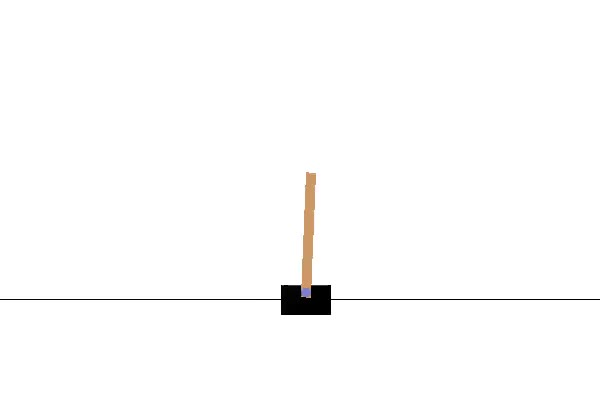
\includegraphics[width=0.4\textwidth]{cartpole.jpg}

  \caption{Visualization of the Cartpole environment. The aim is to have the policy learn to balance a cartpole without falling over.}
\end{figure}


We use the implementation of TRPO in RLLab, a package put out by Schulman and others at UC Berkeley and OpenAI. We optimize the step size hyperparameter with Spearmint, an open-source package put out by Snoek et al. as described in their paper. We decide to use the maximum average discounted return over all the rollouts, which may play into the results we get.

% The reinforcement learning environment is Cartpole, provided by OpenAI Gym. The default step size for TRPO is 0.01, so We choose to let the Gaussian process optimization carried out by Spearmint to vary over stepsize ranging from 0.01 to 0.5. Each rollout is run for 40 iterations.

\begin{figure}[H]
  \centering
  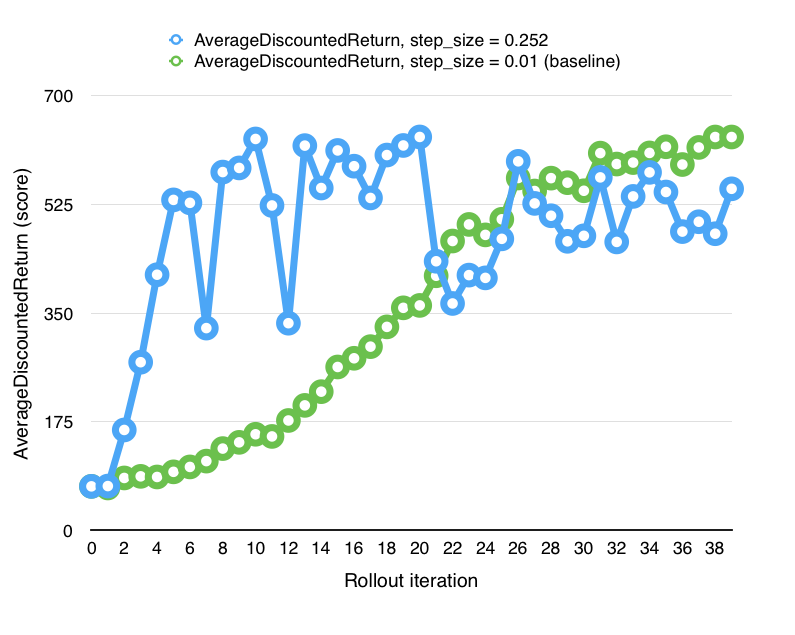
\includegraphics[width=0.5\textwidth]{new_results.png}

  \caption{Comparison with baseline. As you can see, the larger step size allows much more rapid learning in the beginning, but comes as a cost: much of the theoretical work that guarantees monotonic improvement seems to be disregarded by the enormous trust region. It may be that the early success of this algorithm will not scale to larger problems where it is not so easy to improve the policy with large steps.}
\end{figure}


\begin{figure}[H]
  \centering
  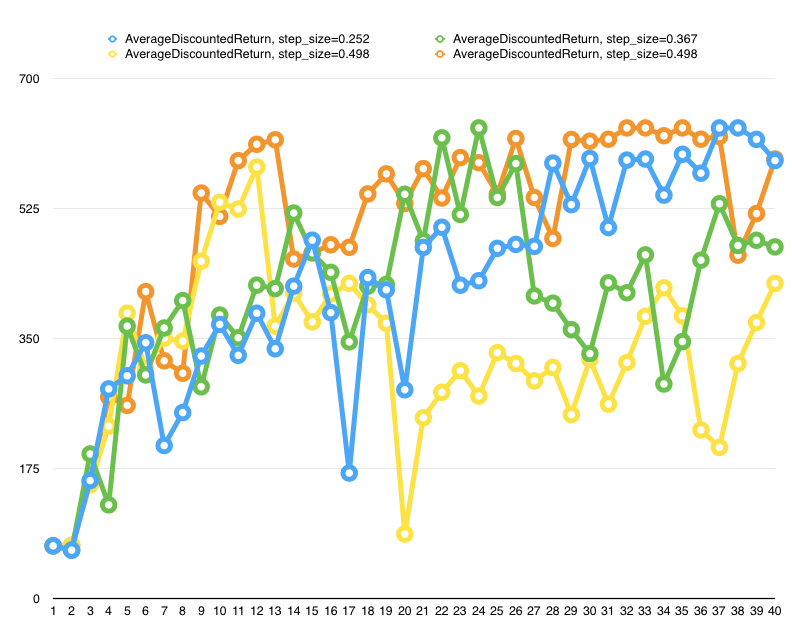
\includegraphics[width=0.5\textwidth]{results.png}

  \caption{Average discounted return over time for various step sizes chosen by the algorithm.}
\end{figure}


As we can see, the discounted return gradually gets better in just a few runs as the Bayesian optimization of the step size approaches the optimal value, which is incidentally better than the default 0.01 early on. However, it is clear that the variance of the average return varies wildly, and it may be that the gains made by the hyperparameter optimization do not generalize to larger policy states.

\section{Conclusion}

Bayesian optimization of TRPO hyperparameters is an early approach. We see reasonably promising results regarding quick learning in the beginning, but much of it seems to undermine the monotonic improvement guarantees. A major factor may be the loss function, which rewards maximum average discounted return (maximized over all rollouts for the specific setting of the hyperparemeter). Future work includes exploring more complicated models for the estimation of the loss function estimation.

\newpage

\begin{thebibliography}{99}

\bibitem{ref1} Schulman, John, et al. "Trust Region Policy Optimization." ICML. 2015.

\bibitem{ref2} Snoek, Jasper, Hugo Larochelle, and Ryan P. Adams. "Practical bayesian optimization of machine learning algorithms." Advances in neural information processing systems. 2012.

\bibitem{ref3} Yan Duan, Xi Chen, Rein Houthooft, John Schulman, Pieter Abbeel. "Benchmarking Deep Reinforcement Learning for Continuous Control". Proceedings of the 33rd International Conference on Machine Learning (ICML), 2016.

\bibitem{ref4} Mnih, Volodymyr, et al. "Human-level control through deep reinforcement learning." Nature 518.7540 (2015): 529-533.

\bibitem{ref5} Brockman, Greg, et al. "OpenAI gym." arXiv preprint arXiv:1606.01540 (2016).

\end{thebibliography}

\end{document}
